\documentclass[12pt,a4paper]{article}
\usepackage[utf8]{inputenc}
\usepackage[english]{babel}

\usepackage{amsmath}
\usepackage{amsfonts}
\usepackage{amssymb}

\usepackage{graphicx}
\usepackage{lmodern}
\usepackage{tikz}
\usepackage{titlesec}
\usepackage{environ}
\usepackage{xcolor}
\usepackage{fancyhdr}
\usepackage[colorlinks = true, linkcolor = black]{hyperref}
\usepackage{xparse}
\usepackage{enumitem}

\usepackage[left=2cm,right=2cm,top=2cm,bottom=2cm]{geometry}
\usepackage{multicol}
\usepackage[indent=0pt]{parskip}

\newcommand{\spaceP}{\vspace*{0.5cm}}
\newcommand{\Span}{\mathrm{Span}\,}
\newcommand{\range}{\mathrm{range}\,}
\newcommand{\ra}{\rightarrow}

%% Redefining sections
\newcommand{\sectionformat}[1]{%
    \begin{tikzpicture}[baseline=(title.base)]
        \node[rectangle, draw] (title) {#1};
    \end{tikzpicture}
    
    \noindent\hrulefill
}

% default values copied from titlesec documentation page 23
% parameters of \titleformat command are explained on page 4
\titleformat%
    {\section}% <command> is the sectioning command to be redefined, i. e., \part, \chapter, \section, \subsection, \subsubsection, \paragraph or \subparagraph.
    {\normalfont\large\scshape}% <format>
    {}% <label> the number
    {0em}% <sep> length. horizontal separation between label and title body
    {\centering\sectionformat}% code preceding the title body  (title body is taken as argument)

%% Set counters for sections to none
\setcounter{secnumdepth}{0}

%% Set the footer/headers
\pagestyle{fancy}
\fancyhf{}
\renewcommand{\headrulewidth}{0pt}
\renewcommand{\footrulewidth}{2pt}
\lfoot{P.-O. Paris{\'e}}
\cfoot{MATH 302}
\rfoot{Page \thepage}

%% Defining example environment
\newcounter{example}[section]
\NewEnviron{example}%
	{%
	\noindent\refstepcounter{example}\fcolorbox{gray!40}{gray!40}{\textsc{\textcolor{red}{Example~\theexample.}}}%
	%\fcolorbox{black}{white}%
		{  %\parbox{0.95\textwidth}%
			{
			\BODY
			}%
		}%
	}

% Theorem environment
\NewEnviron{theorem}%
	{%
	\noindent\refstepcounter{example}\fcolorbox{gray!40}{gray!40}{\textsc{\textcolor{blue}{Theorem~\theexample.}}}%
	%\fcolorbox{black}{white}%
		{  %\parbox{0.95\textwidth}%
			{
			\BODY
			}%
		}%
	}
	

%%%%
\begin{document}
\thispagestyle{empty}

\begin{center}
\vspace*{2.5cm}

{\Huge \textsc{Math 302}}

\vspace*{2cm}

{\LARGE \textsc{Chapter 4}} 

\vspace*{0.75cm}

\noindent\textsc{Section 4.4: Autonomous Second Order Equations}

\vspace*{0.75cm}

\tableofcontents

\vfill

\noindent \textsc{Created by: Pierre-Olivier Paris{\'e}} \\
\textsc{Fall 2022}
\end{center}

\newpage

\section{Undamped Spring-Mass System}

\begin{example}
Consider an object with mass $m$ suspended from a spring and moving vertically freely (in the void). Let $y$ be the displacement of the object from the position it occupies when suspended at rest from the spring. \begin{enumerate}
\item Use Newton's Second Law of motion and Hook Law for springs to find a differential equation describing $y(t)$.
\item Solve this differential equation.
\end{enumerate}
\end{example}

\newpage

\phantom{1}

\newpage

\section{Autonomous ODEs}
A second order ODE that can be written as
	\begin{align}
	y'' = F (y, y') \label{Eq:AutonomousODE}
	\end{align}
where $F$ is independent of $t$, is said to be \textbf{autonomous}.

\underline{Trick to convert to a first order ODE}:

\vfill

\subsection{Undamped Autonomous ODE}
We will be interested in this particular \textbf{undamped autonomous ODE}:
	\begin{align}
	y'' + p(y) = 0 \label{Eq:ParticularAutODE}
	\end{align}
which can be transformed, with the trick, into the first order ODE
	\begin{align}
	v \frac{dv}{dy} + p(y) = 0 \label{Eq:ParticularPhasePlaneAut}.
	\end{align}
	
\underline{Solution:}

\subsection{General Terminology}
\begin{itemize}
\item The ODE \eqref{Eq:ParticularPhasePlaneAut} is called the \textbf{phase plane equivalent} of \eqref{Eq:ParticularAutODE}.
\item The plane with axes $y$ and $v$ is called the \textbf{Poincaré phase plane} of the ODE \eqref{Eq:ParticularPhasePlaneAut}
\item The integral curves of the ODE \eqref{Eq:ParticularPhasePlaneAut} are called \textbf{trajectories}.
\item If a constant $c$ is such that $p(c) = 0$, then
	\begin{itemize}
	\item We say that $y = c$ is an \textbf{equilibrium} of \eqref{Eq:ParticularAutODE}.
	\item We say that $(c, 0)$ is a \textbf{critical point} of \eqref{Eq:ParticularPhasePlaneAut}.
	\end{itemize}
\end{itemize}

\newpage

\section{The Undamped Pendulum}

\begin{example}
Consider the motion of a pendulum with mass $m$, attached to the end of a weightless rod with length $L$ rotating on a frictionless axle. We assume there's no air resistance. The ODE describing the angle $y$ is
	\begin{align*}
	mL y'' = -mg \sin y .
	\end{align*}
	\begin{enumerate}
	\item Solve this ODE with the additional assumption that $v = v_0$ at $y = 0$.
	\item Find the critical points of this ODE.
	\item Study the behavior when $|v_0| > 2 \sqrt{g/L}$.
	\item Study the behavior when $0 < |v_0| < 2 \sqrt{g/L}$.
	\end{enumerate}
\end{example}

\newpage

\phantom{2}

\newpage


\begin{figure}
\centering
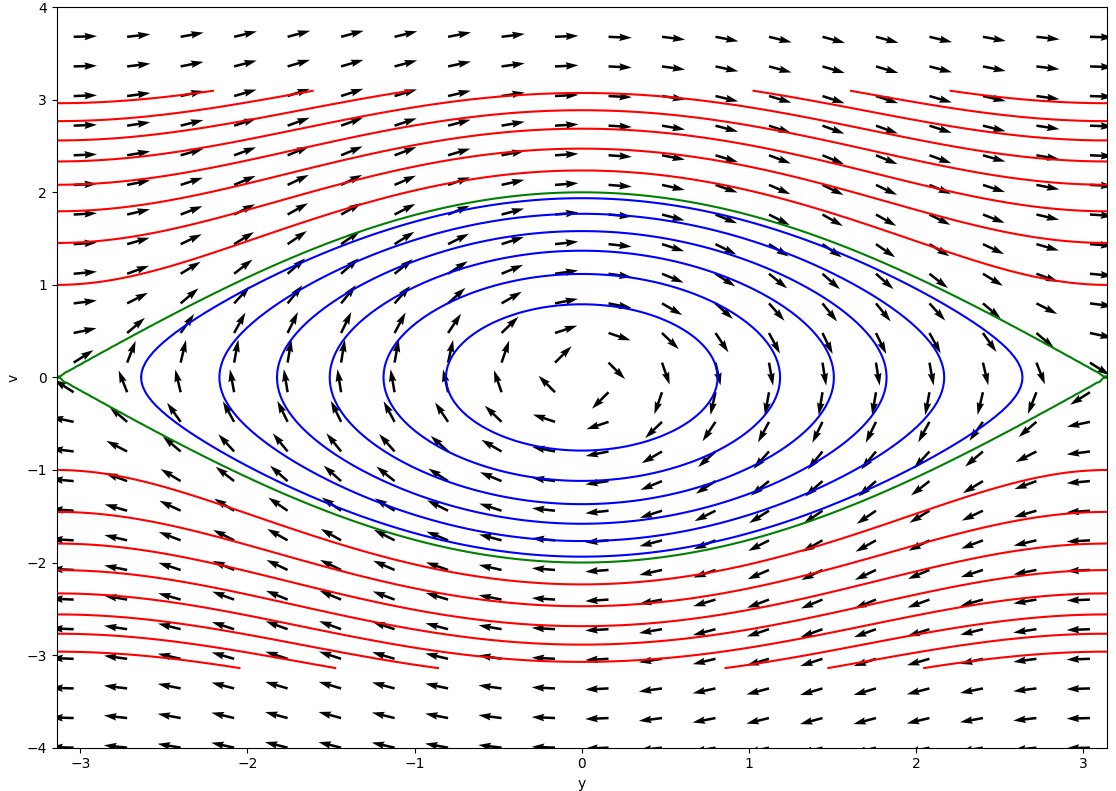
\includegraphics[scale=0.575]{PhaseSpace-UndampedPendulum.png}
\caption{Phase space of the undamped pendulum ODE and some trajectories}\label{Fig:PhaseSpaceUndampedPendulum}
\end{figure}

\underline{Remark:}

	\begin{itemize}
	\item the curves in the phase plane that separates trajectories of whirling solutions (in \textcolor{red}{red}) from the trajectories of oscillating solutions (in \textcolor{blue}{blue}) are called \textbf{separatrix} (in \textcolor{green}{green}).
	\item For a detail study of the stability/unstability behavior of the undamped equation \eqref{Eq:ParticularPhasePlaneAut}, you may read the pages 170-172 of the textbook.
	\item For a study of the damped ODE
		\begin{align*}
		y'' + q (y, y') y' + p(y) = 0,
		\end{align*}
	you may read pages 172-175 of the textbook.
	\end{itemize}


\end{document}